\documentclass{article}
\usepackage[utf8]{inputenc}
\usepackage{tikz}
\usepackage{bchart}
\usepackage{pgfplots,pgfplotstable}\pgfplotsset{compat=1.9}
\usetikzlibrary{external}
\tikzexternalize[prefix=tikz/]

\pgfplotstableread[col sep = comma]{Validation.csv}\Validation
\pgfplotstableread[col sep = comma]{blm-20-final1.csv}\blm
\pgfplotstableread[col sep = comma]{ilm-20-final1.csv}\ilm
\pgfplotstableread[col sep = comma]{seq-length.csv}\seq
\title{SunilGraph}
\author{Steven Goldenberg}
\date{February 2019}

\begin{document}
\maketitle

\section{Introduction}
 
\begin{figure}
    \centering
    \begin{tikzpicture}
    \begin{axis}[
        align={center}, 
        xmin=0,
        height = 0.5\textwidth,
        width = \textwidth,
%        #xtick={1,2,3,4,5,6,7,8,9,10}, 
        ytick={0,10,...,110},
        title = NGram vs Average Perplexity,
        xlabel = NGram,
        ylabel = Avg. Perplexity,
        nodes near coords={\pgfmathprintnumber[precision=1]{\pgfkeysvalueof{/data point/y}}},
        every node near coord/.append style={font=\footnotesize},
        every axis plot/.append style={semithick}
        ]

    \addplot[blue,opacity=0.9,mark=x] table[x=NGram, y=Average Perplexity]{\blm};

	\end{axis}
    \end{tikzpicture}
    
    \caption{10-Fold Cross Validation with Backoff Method}
    \label{fig:my_label}
\end{figure}

d
\begin{figure}
    \centering
    \begin{tikzpicture}
    \begin{axis}[
        align={center}, 
        xmin=0,
        height = 0.5\textwidth,
        width = \textwidth,
%        #xtick={1,2,3,4,5,6,7,8,9,10}, 
        %ytick={0,10,...,110},
        title = 10-Fold Cross Validation with Backoff Method,
        xlabel = NGram,
        ylabel = Cross Entropy,
        nodes near coords={\pgfmathprintnumber[fixed,precision=3]{\pgfkeysvalueof{/data point/y}}},
        every node near coord/.append style={font=\footnotesize},
        every axis plot/.append style={semithick}
        ]

    \addplot[blue,opacity=0.9,mark=x] table[x=NGram, y=Cross-Entropy]{\blm};

\end{axis}
    \end{tikzpicture}
    
    \caption{NGram VS Cross Entropy Or some explanation}
    \label{fig:my_label}
\end{figure}


\begin{figure}
    \centering
    \begin{tikzpicture}
    \begin{axis}[
        align={center}, 
        xmin=0,
        height = 0.5\textwidth,
        width = \textwidth,
%        #xtick={1,2,3,4,5,6,7,8,9,10}, 
        ytick={0,10,20,30},
        title = NGram vs Average Perplexity,
        xlabel = NGram,
        ylabel = Avg. Perplexity,
        nodes near coords={\pgfmathprintnumber[precision=1]{\pgfkeysvalueof{/data point/y}}},
        every node near coord/.append style={font=\footnotesize},
        every axis plot/.append style={semithick}
        ]

    \addplot[blue,opacity=0.9,mark=x] table[x=NGram, y=Average Perplexity]{\ilm};

\end{axis}
    \end{tikzpicture}
    
    \caption{10-Fold Cross Validation with Interpolation Method}
    \label{fig:my_label}
\end{figure}

\begin{figure}
    \centering
    \begin{tikzpicture}
    \begin{axis}[
        align={center}, 
        xmin=0,
        height = 0.5\textwidth,
        width = \textwidth,
%        #xtick={1,2,3,4,5,6,7,8,9,10}, 
        %ytick={0,10,...,110},
        title = 10-Fold Cross Validation with Interpolation Method,
        xlabel = NGram,
        ylabel = Cross Entropy,
        nodes near coords={\pgfmathprintnumber[fixed,precision=3]{\pgfkeysvalueof{/data point/y}}},
        every node near coord/.append style={font=\footnotesize},
        every axis plot/.append style={semithick}
        ]

    \addplot[blue,opacity=0.9,mark=x] table[x=NGram, y=Cross-Entropy]{\ilm};

\end{axis}
    \end{tikzpicture}
    
    \caption{\large 10-Foldd Crossd Validation with Interpolation Method}
    \label{fig:my_label}
\end{figure}


\begin{figure}
    \centering
    \begin{tikzpicture}
    \begin{axis}[
		legend cell align={left},
        align={center}, 
        xmin=0,
        ymax=20,
        height = 0.8\textwidth,
        width = \textwidth,
		xtick={1,2,...,10}, 
        ytick={0,4,...,16},
        %title = Different Methods,
        xlabel = n-gram,
        label style={font=\Large},
        tick label style={font=\Large},
        ylabel = Self Cross-Entropy in bits,
       % nodes near coords={\pgfmathprintnumber[fixed,precision=3]{\pgfkeysvalueof{/data point/y}}},
       % every node near coord/.append style={font=\footnotesize},
        every axis plot/.append style={thick}
        ]
    \addplot[green!30!black,mark=triangle*,mark size=3pt] table[x=NGram, y=Cross-Entropy]{\ilm};
     \addlegendentry{HOME Corpus}

    \addplot[teal,opacity=0.9,mark=square,mark size=3pt] table[x=NGram, y=C-sharp Raw]{\ilm};
     \addlegendentry{C\# Raw Data}

    \addplot[blue,mark=asterisk,mark size=3pt] table[x=NGram, y=C-sharp without Syntax Tokens]{\ilm};
     \addlegendentry{C\# without Syntax Tokens}

    \addplot[black,mark=o,mark size=3pt] table[x=NGram, y=Gutenberg]{\ilm};
     \addlegendentry{Gutenberg Corpus}

\end{axis}
    \end{tikzpicture}
    \caption{\large{10-Fold Cross Validation with Interpolation Method- All}}
    \label{fig:my_label}
\end{figure}


\begin{figure}
    \centering
    \begin{tikzpicture}
    \begin{axis}[
		legend cell align={left},
        align={center}, 
        xmin=0,
        ymax=16,
        height = 0.8\textwidth,
        width = \textwidth,
		xtick={1,2,...,10}, 
        ytick={0,4,...,16},
        %title = Figure 1,
        xlabel = n-gram,
        label style={font=\Large},
        tick label style={font=\Large},
        ylabel = Self Cross-Entropy in bits,
       % nodes near coords={\pgfmathprintnumber[fixed,precision=3]{\pgfkeysvalueof{/data point/y}}},
      %  every node near coord/.append style={font=\footnotesize},
        every axis plot/.append style={thick}
        ]
    \addplot[green!30!black,mark=triangle*,mark size=3pt] table[x=NGram, y=Cross-Entropy]{\ilm};
     \addlegendentry{HOME Corpus}
%{H$\epsilon$lion}
    \addplot[blue,mark=asterisk,mark size=3pt] table[x=NGram, y=C-sharp Raw]{\ilm};
     \addlegendentry{C\# Raw Data}

   % \addplot[blue,opacity=0.9,mark=pentagon] table[x=NGram, y=C-sharp without Syntax Tokens]{\ilm};
    % \addlegendentry{C\# without Syntax Tokens}

    \addplot[black,mark=o,mark size=3pt] table[x=NGram, y=Gutenberg]{\ilm};
     \addlegendentry{Gutenberg Corpus}

\end{axis}
    \end{tikzpicture}
    \caption{\large{10-Fold Cross Validation with Interpolation Method-Raw}}
    \label{fig:my_label}
\end{figure}
\begin{figure}
    \centering
    \begin{tikzpicture}
    \begin{axis}[
		legend cell align={left},
        align={center}, 
        xmin=0,
        ymax=16,
        height = 0.8\textwidth,
        width = 1\textwidth,
		xtick={1,2,...,10}, 
    %    ytick={0,4,...,16},
        %title = Figure 2,
        xlabel = n-gram,
        label style={font=\Large},
        tick label style={font=\Large},
        ylabel = Self Cross-Entropy in bits,
%        nodes near coords={\pgfmathprintnumber[fixed,precision=3]{\pgfkeysvalueof{/data point/y}}},
%        every node near coord/.append style={font=\small},
        every axis plot/.append style={thick}
        ]
    \addplot[green!30!black,mark=triangle*,mark size=3pt] table[x=NGram, y=Cross-Entropy]{\ilm};
    \addlegendentry{HOME Corpus}
%    \addplot[teal,mark=triangle] table[x=NGram, y=C-sharp Raw]{\ilm};
 %    \addlegendentry{C\# Raw Data}
    \addplot[blue,mark=asterisk,mark size=3pt] table[x=NGram, y=C-sharp without Syntax Tokens]{\ilm};
     \addlegendentry{C\# without Syntax Tokens}
    \addplot[black,mark=o,mark size=3pt] table[x=NGram, y=Gutenberg]{\ilm};
     \addlegendentry{Gutenberg Corpus}

\end{axis}
    \end{tikzpicture}
    \caption{{\large 10-Fold Cross Validation evaluated with Interpolation Method -Syntax}}
    \label{fig:my_label}
\end{figure}

% Sequence Length

\begin{figure}
    \centering
    \begin{tikzpicture}
    \begin{axis}[
		legend cell align={left},
        align={center}, 
        xmin=0,
        ymax=16,
        height = 0.5\textwidth,
        width = \textwidth,
		xtick={10,20,...,100}, 
	    %ytick={0,4,...,20},
        %title = Figure 2,
        xlabel = Sequence Length,
        label style={font=\large},
        tick label style={font=\Large},
        ylabel = Self Cross-Entropy in bits,
        nodes near coords={\pgfmathprintnumber[fixed,precision=3]{\pgfkeysvalueof{/data point/y}}},
        every node near coord/.append style={font=\footnotesize},
        every axis plot/.append style={thick}
        ]
    \addplot[green!30!black,mark=triangle*,mark size=3pt] table[x=Sentence Length, y=Cross-Entropy]{\seq};
     \addlegendentry{HOME Corpus}

\end{axis}
    \end{tikzpicture}
    \caption{{\large 10-Fold Cross Validation with different Sequence Lengths}}
    \label{fig:my_label}
\end{figure}



\begin{figure}
    \centering
    \begin{tikzpicture}
    \begin{axis}[
		legend cell align={left},
        align={center}, 
        xmin=0,
        ymax=16,
        height = 0.5\textwidth,
        width = \textwidth,
		xtick={10,20,...,100}, 
	    %ytick={0,4,...,20},
        %title = Figure 2,
        xlabel = Sequence Length,
        label style={font=\large},
        tick label style={font=\Large},
        ylabel = Self Cross-Entropy in bits,
        nodes near coords={\pgfmathprintnumber[fixed,precision=3]{\pgfkeysvalueof{/data point/y}}},
        every node near coord/.append style={font=\footnotesize},
        every axis plot/.append style={thick}
        ]
    \addplot[green!30!black,mark=triangle*,mark size=3pt] table[x=Sentence Length, y=Cross-Entropy]{\seq};
     \addlegendentry{HOME Corpus}

\end{axis}
    \end{tikzpicture}
    \caption{{\large 10-Fold Cross Validation with different Sequence Lengths}}
    \label{fig:my_label}
\end{figure}

\begin{figure}
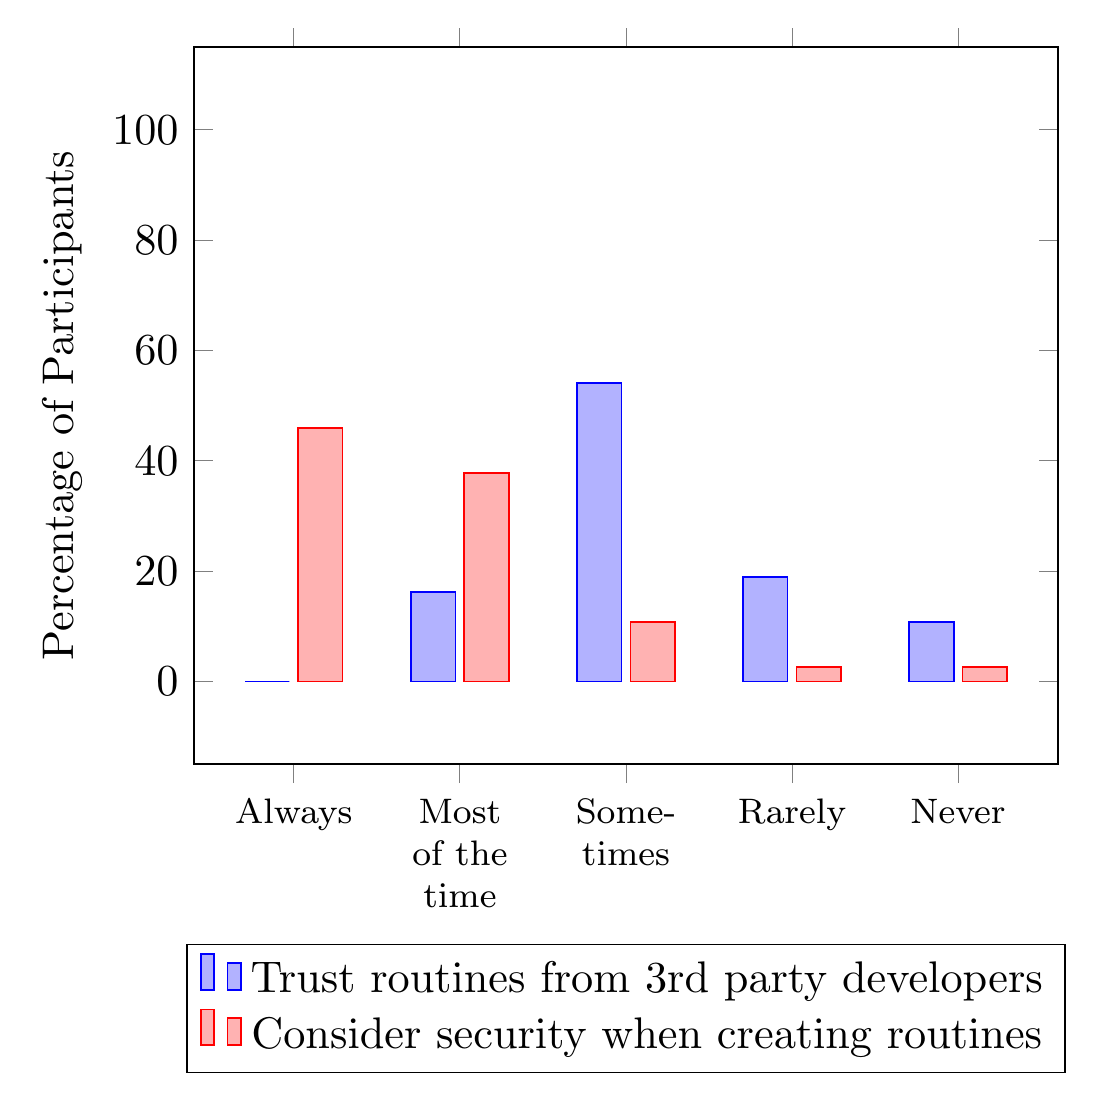
\begin{tikzpicture}[scale=1.6,transform shape]
\begin{axis}[
ybar,
ymax=100,
enlargelimits=0.15,
legend style={at={(0.5,-0.25)},anchor=north},
ylabel={Percentage of Participants},
symbolic x coords={Always,Most of the time,Some-times, Rarely,Never},
xtick=data,
xticklabel style={text width=1.0cm,
font=\footnotesize,
label style={font=\large},
align=center
},
]
%3d party
\addplot[blue,fill=blue!30!white,error bars/.cd,y dir=both,y explicit,]
coordinates{(Some-times,54.05) (Rarely,18.91) (Always,0)  (Most of the time,16.21) (Never,10.81) };
\addlegendentry{Trust routines from 3rd party developers}
%Consider security
\addplot[red,fill=red!30!white,error bars/.cd,y dir=both,y explicit,]
coordinates {(Some-times,10.81) (Rarely,2.70) (Always,45.94)  (Most of the time,37.83) (Never,2.70)
};
%\legend{Consider Security \\when creating routines,Trust Routines by 3rd party developers}
\addlegendentry{Consider security when creating routines}

\end{axis}
\end{tikzpicture}
\caption{Unterschrift}
\label{GedaechtnisBilder}
\end{figure}




\begin{figure}
\begin{tikzpicture}[scale=1.6,transform shape]
\begin{axis}[
ybar,
ymax=100,
enlargelimits=0.15,
legend style={at={(0.5,-0.25)},anchor=north},
ylabel={Percentage of Participants},
symbolic x coords={Always,Most of the time,Some-times, Rarely,Never},
xtick=data,
xticklabel style={text width=1.0cm,
font=\footnotesize,
label style={font=\large},
align=center
},
]
%3d party
\addplot[blue,fill=blue!30!white,error bars/.cd,y dir=both,y explicit,]
coordinates{(Some-times,54.05) (Rarely,18.91) (Always,0)  (Most of the time,16.21) (Never,10.81) };
\addlegendentry{Would you test your routines \\
to make sure they execute you want it to?}
%Consider security
\end{axis}
\end{tikzpicture}
\caption{Unterschrift}
\label{GedaechtnisBilder}
\end{figure}
ds
\end{document}
